\documentclass[a4paper,titlepage]{article}
\usepackage{frontespizio}
\usepackage[english]{babel}
\usepackage[utf8]{inputenc}
\usepackage{usecases}

\usepackage{tikz}
\usetikzlibrary{arrows,shadows} % for pgf-umlsd
\usepackage[underline=true,rounded corners=false]{pgf-umlsd}

\usepackage{enumitem}
\setitemize{noitemsep,topsep=0pt,parsep=0pt,partopsep=0pt}

\usepackage[a4paper, total={6in, 9in}]{geometry}



\begin{document}
\begin{frontespizio}
\Universita{Verona}
\Dipartimento{Informatica}
\Corso[Laurea]{Informatica}
\Titoletto{Software Engineering}
\Titolo{First project report}

\Candidato[VR363021]{Giovanni Liboni}
\Candidato[VR359169]{Enrico Giordano}
\Candidato[VR359129]{Alberto Marini}
\Candidato[VR359333]{Alessandro Falda}

\Annoaccademico{2013-2014}
\end{frontespizio}

\tableofcontents

\newpage

\part{Introduction}

This report explain how a car parking system was implemented by the project group. This project was implemented in java language and the nodes of the system was converted into class, according to object oriented programming. 

~

Every entity was interpreted as a node of a grid that comunicate to another node with a channel; it use a particular node, Tx or Rx, wherewith send or receive messages. This remaind a particular design pattern called ''observer pattern``: it is a software design pattern in which an object, called the subject, maintains a list of its dependents, called observers, and notifies them automatically of any state changes, usually by calling one of their methods. It is mainly used to implement distributed event handling systems.

Every entity was a generalization of an abstract class called Node; infact an entity of system is a specialization of Node class. This fact remaind an embedded system which is composed by a simple hardware objects that comunicate each other and send or receive messagges. 

\newpage
\part{General pattern}

Now it's explain an example of system behaviour: when a car arrive or exit to the park, the node ''car detector`` send a message to the node ''process unit``, that store the request (for future use) and send to the monitor the average number of car/hour and the number of free parking places. 

According to observer pattern, the subject (Sensor) notify the observer (Process Unit) that a new message is pending, so observer (Process Unit) receive istantly the message. After the computation, the Process Unit send in the same way the messages to the different displays.
The observer pattern is used only in the comunication nodes.

So the sender node, when have to send a message, must call the receive method of the receiver node; in this way it was implemented an observer pattern, an optimization of a real system. In fact, in a real context, the receiver must poll on the receive path (or hardware) or must have an interrupt routine that manage the receiving process; in this system, the sender simply call a receive method of the receiver.

In the picture, the arrows show how a class (or a method) call other class. 

    \begin{center}

    \centering
    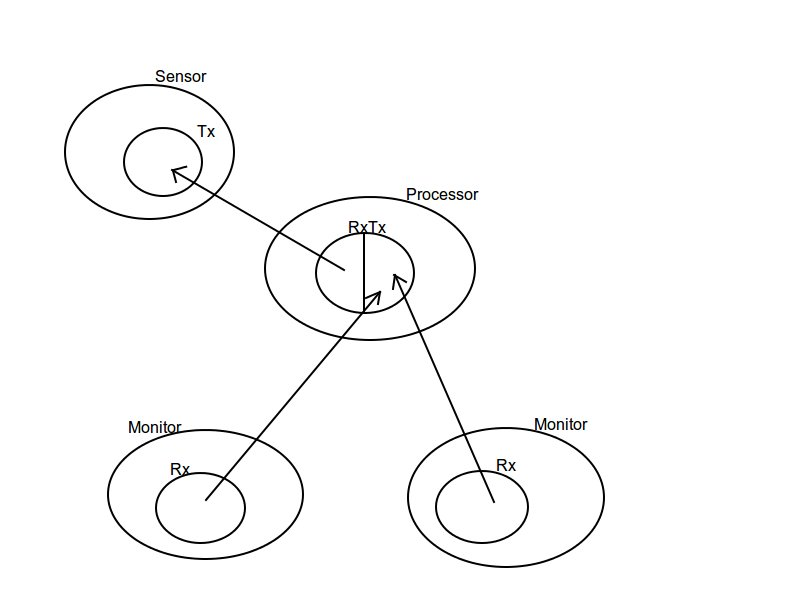
\includegraphics[scale=0.40]{pattern.jpg}

    \end{center}


There is a different type of node in this project, in particular:

\begin{itemize}[noitemsep,topsep=20pt,parsep=10pt,partopsep=20pt]

\item Detector: a sensor that controls car traffic (entering or exiting car); 
\item Processor: a processing unit that calculate average number of cars/hour anche number of free parking places;
\item Monitor: a display that shows the results of processing unit.

\end{itemize}

The channel comunication was implemented by ''Channel`` class, that create a link in a comunication grid. There are 2 tipes of Channel: WireChannel or WirelessChannel (in this project there is no difference).

The Processor computation is done by a subnode called nodeComputation, that implement basic operation (sum, min, ecc...). A complex computation is formed by a combination of basic operation, like an ALU of a real processor.

The comunication is done by a subnode called nodeCommunication, that implement:

\begin{itemize}[noitemsep,topsep=20pt,parsep=10pt,partopsep=20pt]

\item TxNode: must send a message (for Detector);

\item RxNode: must receive a message (for Monitor);

\item TxRxNode: must send and receive a message (for Processor);

\end{itemize}

It was used a Strategy pattern for implementation of nodes, because there is an ``abstract'' class and other classes is an implementation of this class. Every class inheredits methods and attribute from abstract node and implements it. 

When a node send a message, it set the receiver channel and send to it using the right channel.

\newpage
\part{Simulation}

In the main class is created the detector, the processing unit and 3 monitor: a display for average number of car/hour, a display for number of free parking places and an (not required) display for car traffic.

The node is linked in the wireless grid and, after that, they can comunicate. A realtime clock in the processing unit simulate the time (for the average cars/hours) implemented with a thread that every second increase a counter. 

\section*{GUI}

It was implemented a simple user interface that simulate a scenario of the system. There are:

\begin{itemize}

\item a control button panel, which contains three buttons (start, stop, reset) that controll intuitively the system;
\item a complex of simple monitor that show the evolution of the system.

\end{itemize}

With the control button, the user can control the simulation: ``start'' button starts the simulation, ``stop'' button stops the simulation and ``restart'' button restarts the simulation.

    \begin{center}

    \centering
    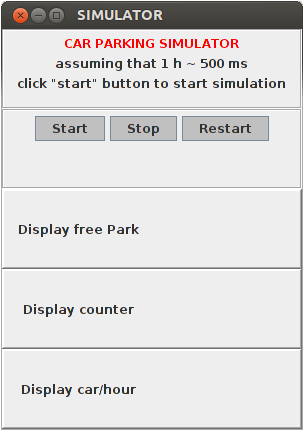
\includegraphics[scale=0.50]{interface.png}

    \end{center}

Every node of the system is brother to each other node and can comunicate using reference of the node class, known by the superclass.


\newpage
\part{Questions}

\section*{ Which patterns are used within the scheme of Figure 2?}

The first figure represents an interface class called ``nodeCommunication'' and three other classes (TxNode, RxNode and TxRxNode) that implement the nodeCommunication interface. The interface class is a type of class that presents many methods of a particular class; this methods are not implemented, but the class that implements this interface must implements them.

~

The second figure represents an another interface called ``nodeComputation'' and some other classes (Add, Sub, Average, Divide, Multi, Comparator) that implement nodeComputation interface. Every nodeComputation class must have a method that must be implemented by the programmer. Interfaces cannot be instantiated, but rather are implemented. A class that implements an interface must implement all of the methods described in the interface, or be an abstract class. They simulate multiple inheritance.

~

The third figure represents an abstract class called ``Node'' and three other class (Detector, Processor, Monitor) that inherited the superclass methods (``Node''). The abstract class must have some implemented method and the son classes have the same method and the same attribute. If a son classes have a different implementation of a method, it must override it.  

An abstract type may provide no implementation, or an incomplete implementation. Abstract types will have one or more implementations provided separately, like in this case. 

~

So this is a Strategy Pattern. The strategy pattern is a software design pattern that enables an algorithm's behavior to be selected at runtime. For instance, a class that performs validation on incoming data may use a strategy pattern to select a validation algorithm based on the type of data, the source of the data, user choice, or other discriminating factors. These factors are not known for each case until run-time, and may require radically different validation to be performed. The validation strategies, encapsulated separately from the validating object, may be used by other validating objects in different areas of the system (or even different systems) without code duplication.

\newpage
\section*{Explanation of used patterns}

    \begin{center}

    \centering
    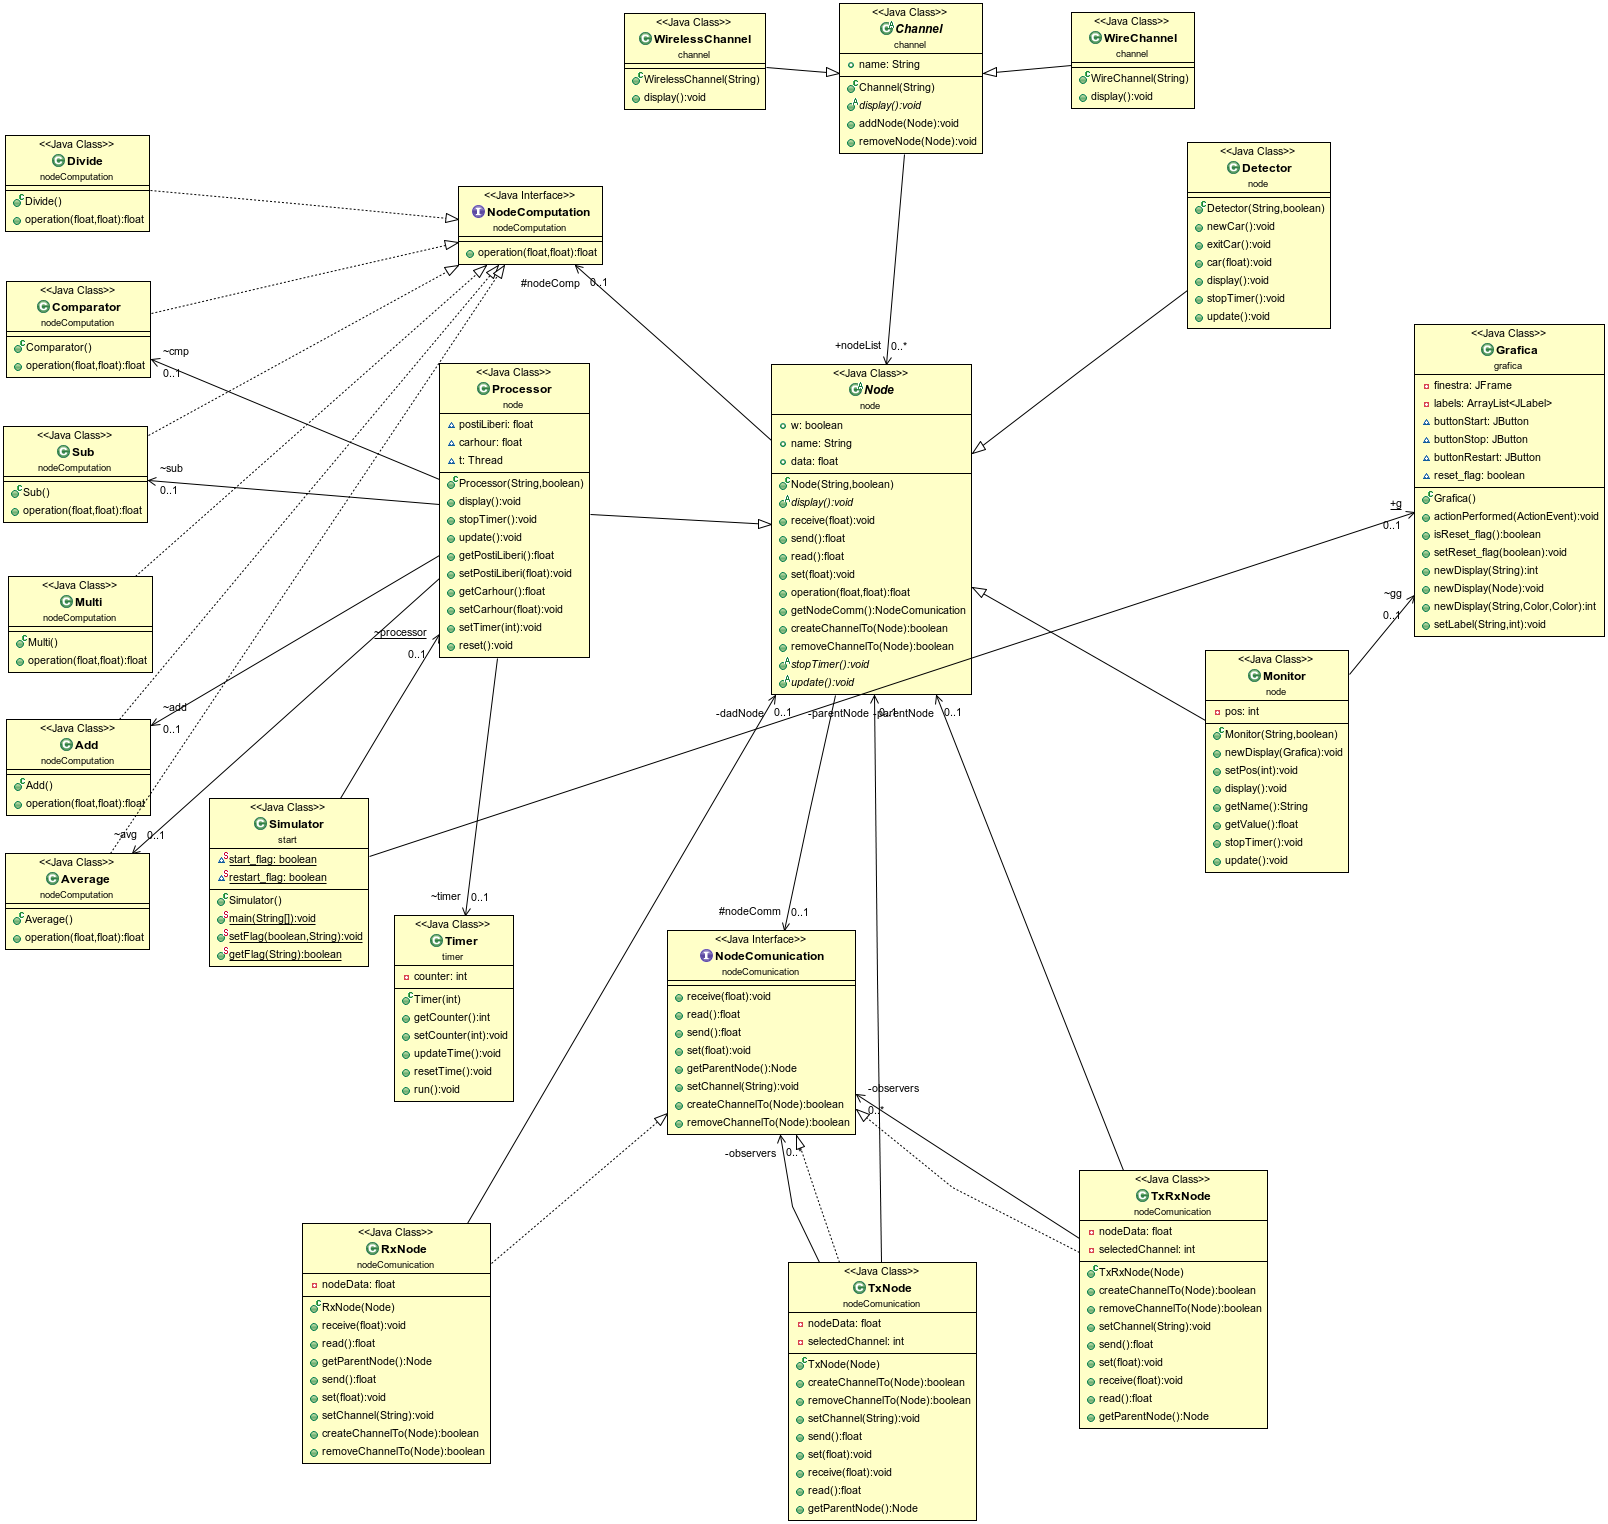
\includegraphics[scale=0.30]{ClassDiagram.png}

    \end{center}


The first class, Simulator, can instantiate the other class of the system. Every node is chained to the other by a wireless grid and can comunicate thanks to the observer pattern, using a ``subnode'' called Tx (for trasmission), Rx (for receiving) and TxRx (both). There is a graphical interface that is accessible by all classes. The ``actors'' of the system (Detector, Monitor, Detector, Processor) are an implementation of Node class.


\end{document}


